\documentclass[a4paper,11pt]{article}
\usepackage{fullpage}

\usepackage{subfigure}
\usepackage{enumitem}
\usepackage{graphicx}
\usepackage{amsmath}
\usepackage{amssymb}
\usepackage{amsthm}
\newtheorem{theorem}{Theorem}[section] 
\usepackage{pgf}
\usepackage{float}
\usepackage{multicol}
\usepackage[utf8]{inputenc}
\usepackage[english]{babel}
\usepackage[toc,page]{appendix}

\newcommand{\code}[1]{\texttt{#1}}
\setlength{\columnsep}{1cm}


\DeclareMathAlphabet{\mathpzc}{OT1}{pzc}{m}{it}


\newtheorem{definition}{Definition}


\let\cleardoublepage\clearpage
\usepackage{todonotes}
\newcommand{\TJ}[1]{\todo[color=green!50]{\sf \textbf{TJ:} #1}}
\newcommand{\TAP}[1]{\todo[inline,color=red!50]{\sf \textbf{TAP:} #1}}
\newcommand{\MQ}[1]{\todo[inline,color=blue!50!red!10]{\sf \textbf{MQ:} #1}}





\usepackage{multidef}
\usepackage{xspace}
\multidef[prefix=bb]{\mathbb{#1}\xspace}{A-Z,One->1}
\multidef{\textsf{#1}}{Actors,Network,Synchronization,Mailboxes,Communications,mailbox,communication,Mutexes}
\multidef{\textsf{\textit{#1}}\xspace}{send,receive,mutexlock->MutexAsyncLock,mutexunlock->MutexUnlock,mutexwait->MutexWait,mutextest->MutexTest, localcomputation->LocalComputation, asynsend->AsyncSend, asynreceive->AsyncReceive, test->Test, wait->Wait, localcompute->LocalComputation}


\title{Formal Semantics of the SimGrid Simulator}
\begin{document}
\maketitle

This document tries to formally express the semantic of applications that can be executed in SimGrid, such as MPI applications. The long term goals is to find better reduction algorithms for MPI applications in Mc SimGrid, the model-checker embedded within the SimGrid framework.

\medskip

SimGrid is a simulator of distributed applications. Several user interfaces are proposed, ranging from the classical and realistic MPI formalism, to less realistic simgrid-specific APIs that ease the expression of theoretical distributed algorithms. These user interfaces are built upon a common interface, that is implemented either on top of a performance simulator, or on top of a model-checker exploring exhaustively all possible outcomes from a given initial situation.

\centerline{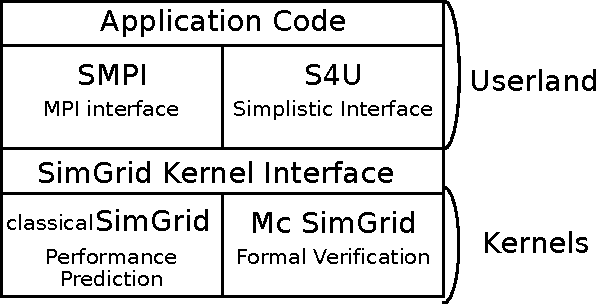
\includegraphics[scale=.6]{simgrid-architecture.pdf}}

The distributed application is represented in SimGrid as a set of \textbf{actors}, representing  
processes or threads of real applications, or MPI ranks. These actors  interact with each other either through message passing, or with classical synchronization objects (such as mutexes or semaphores), or through executions on CPUs and read/write  operations on disks.

Even if it simulates distributed applications, SimGrid proposes a shared memory model: all actors share the same memory space. To simulate distributed settings, most of the simulated applications simply ensure that they only use variables that are local to each actor, without any program global variables. Enforcing the memory separation at application level allows the kernel to deal with shared-memory and distributed-memory primitives in the same way. It also permits to partially abstract the studied simulated infrastructure: the distributed services that are not relevant to the study can easily be abstracted as centralized components.

From the formal point of view, a major advantage of the SimGrid framework is that all user interfaces are implemented on top of a very small amount of kernel primitives.
In this document, we are interested in formalizing these operations and their inter-dependencies, that will be useful for partial-order reduction methods  in model-checking.

\medskip
This document is organized as follows. Section~\ref{sec:sysdef} formally defines the interface offered by the SimGrid kernel. It specifies the semantic of every offered operation types through their effects on the system. Section~\ref{sec:eventsystem} defines an event system with these operations, exploring the causality, conflict and independence relations between the defined events. Section~\ref{sec:mpi} presents how the MPI semantic is implemented on top of the SimGrid kernel. 

\MQ{Here comes the figure you've done on my board, explaining how we will build an unfolding structure, along with the text briefly explaining the corresponding steps, and linking to the corresponding sections}
%%%%%%%%%%%%%%%%%%%%%%%%%%%%%%%%%%%%%%%%%%%%%%%%%%%%%%
\section{System State Definition}\label{sec:sysdef}
A distributed system is a tuple $P=\langle \Actors, \Network, \Synchronization \rangle$ in which  $\Actors$ = $\{ A_1, A_2, ... A_n\}$ is a set of $n$ actors. Actors do not have a global shared memory nor a global clock. The execution of an actor $A_i$ consists of an alternate sequence of local states and actions $s_{i,0}\xrightarrow{\text{$a_0$}} s_{i,1} \xrightarrow{\text{$a_1$}}s_{i,2} ... \xrightarrow{\text{$a_{n-1}$}}s_{i,n}$ (firing $a_i$ from local state $s_{i}$, the local state of the actor $A_i$ changes from $s_i$ to $s_{i+1}$).
All the actions in one actor are totally ordered by the causal relation (see below) \TJ{this will be discussed later ?}. \Network~is considered as a subsystem providing facilities for the \Actors~able exchange messages with each other while \Synchronization~composed of several mechanisms to synchronize actors when they are accessing shared resources. 

\subsection{Network Subsystem}
\MQ{Start from the TLA definitions, and describe it in english afteward if you want. But the TLA def is mandatory! First describe the state (copy/paste TLA + add needed english explainations), and then describe every possible action (or is it API element? Or event? Need to call it the same way everywhere)}

The state of the network subsystem is defined as a pair $\langle \Mailboxes, \Communications \rangle$, where \begin{itemize}[noitemsep]
\setlength{\itemsep}{3pt}
\item $\Mailboxes = \{ \mailbox_1, \mailbox_2, ... \mailbox_m \}$ is a set of $m$ mailboxes, each $\mailbox_i$ is an infinite queue storing $\send$ and $\receive$ requests of agents, it is considered as a rendez-vous
where $\send$ and $\receive$ requests meet. For a given mailbox, corresponding requests are stored with a FIFO policy. It means that when a $\send$ request coming to the mailbox, the oldest $\receive$ is selected to combine with the coming $\send$, producing a ready communication in \Communications~ (the same process for receive requests). Hence, at the same time there are only one kind of pending requests: send or receive requests. The state of the mailbox is indicated by the pending $\send$ or $\receive$ requests. \textcolor{red}{Formally, the state of a mailbox is presented by a pair $\langle n,type \rangle$ where n $\in \mathbb{N}$ is the number of pending requests while type $\in$ \{ "\send" ,"\receive"\} expresses the kind of the requests. Therefor, the $\mailbox's$ state is changed if there is an actor sending a $\send$ or $\receive$ request to it. We use the notion state of the $\Mailboxes$ to imply a m-tupe containing state of all mailboxes. }
\item $\Communications$ is a set of individual communications, each of them describing a data exchange  between two actors.  A $\communication$ with the "ready" status is formed when a $\send$ request matches with a $\receive$ request in a particular mailbox. While a "ready" \communication is ready for exchanging data between two actors, a communication whose status is "\send" or "\receive" is waiting for the supplement information to create a complete communication (ready communication).\textcolor{red}{ The state of the \Communications~is represented by the communications stored inside it. }
\end{itemize}
Four actions are defined in \Network~subsystem to support actors communicate with each other. They are \asynsend, \asynreceive, \wait~ and \test. An actors start a communication by firing a \asynsend~ or \asynreceive; however, data are really exchanged betwen two actors because of firing \wait~ or \test.
\begin{itemize}[noitemsep]
\setlength{\itemsep}{3pt}
\item An actor drops an asynchronous \send~ request to a particular mailbox by firing an \asynsend~ action. If there are pending \receive~ requests in the mailbox, the \send~ request will be matched with the oldest receive request to form a \communication~ with "ready" status in the \Communications. In the other hand, there is no pending receive in the mailbox, the request is stored in the mailbox and a \communication~ is still created in the \Communications~ with a "send" status.  Similarly, actors use \asynreceive~ to post an asynchronous receive on a mailbox; the way a receive request is processed is the same as the way a send request is treated. 

\item Although communications are established in the \Communications~ by the combination of \send~ and \receive~ requests, data are really transferred between actors by firing \test~ or \wait. \test~ returns either true or false depending on the status of the \communication~ what the \test's actor want to test. If the status is "ready" or "done", it returns true, otherwise false is given. As stated, data exchange is performed in \test~ command. In the case where the status is "ready", data is copied from the souse actor to the destination actor, and the status of the communication is assigned to "done". Similarly, \wait~ action has the same function in transferring data, but  it does not return any values, and it can blocks it's actor if the \communication~ is not ready for being processed.   
\end{itemize}

\subsection{Synchronization subsystem}
\MQ{Same here: build everything around the TLA definitions}
The state of the \Synchronization~ subsystem is defined by \Mutexes
\begin{itemize}[noitemsep]
\setlength{\itemsep}{3pt}
 \item 
  $\Mutexes$ = $\{m_1, m_2 ... m_k \}$ is a set of k asynchronous mutexes. The $\Mutexes$ are used to synchronize the actors. An actor $A_i$ declares it's interest on a mutex $m_j$ by executing the action $\mutexlock(A_i,m_j)$~  while the mutex remembers that interest by adding the id of the actor to it's waiting queue. This queue also follows a FIFO policy. An actor is considered the {\em owner} of a mutex if it is the first in the mutex's waiting queue while the others in the queue are [\em waiting] actors. We say that a mutex $m$ is {\em busy} if there is at least one actor in it's waiting queue, otherwise it is {\em free}.\textcolor{red}{ The state of the $\Mutexes$ is indicated by state of all the mutexes, more formally the state of $\Mutexes$ = $\{state1, state_2 ... state_k \}$ where $state_i$ $\in$ \{"free", "busy" \} }
 \end{itemize}

 In this model mutexes are asynchronous, similar to communication, in the sense that requesting a mutex is not blocking. 
 In the synchronization subsystem, there are four actions  allowing actors to interact with the \Mutexes, namely \mutexlock, \mutexunlock, \mutexwait~ and \mutextest, where  
 \begin{itemize}[noitemsep]
\setlength{\itemsep}{3pt}
 \item $\mutexlock(A_i,m_j)$~ is executed by an actor $A_i$ when the actor wants to acquire a mutex $m_j$. After firing \mutexlock, the id $i$ of the actor will be added to the tail of the mutex's queue. If the mutex was free, the actor becomes the owner of the mutex, and to help the actor identify which mutexes it has asked for, the mutex's id $j$ is added to it's requests set \TJ{add this in the actors state?}. Unlike classical mutexes, when an actor is waiting for a mutex, it is not blocked.
\item \mutexunlock~ is used to remove an interest on a mutex by an actor. Either the actor is the owner or not, this command can be fired by the mutex, deleting the id of the actor from the mutex's queue and removing the mutex's id from actor's request set. 
\item An actor can check if it is the owner of a mutex that he has previously asked for access to (id of the mutex is included in the actor's request set). To realize this, it can use the \mutextest~action, returning true if the id of the actor is the first element of the mutex's waiting queue, otherwise the returned value is false. While a \mutextest~ can be fired at any time, a \mutexwait~ can only be executed by an actor when the actor owns the mutex. Hence, a waiting actor can be blocked when trying to execute \mutexwait. 
 \end{itemize}

\subsection{Summary}
Actor = local state (containing variables and PC) + program (sequence of actions) 

\noindent\centerline{\begin{tabular}{|c||c|c|}\hline
 \textbf{Subsystem}&\Network&\Synchronization\\\hline\hline
 %
 \textbf{Resource}&Mailbox& Mutex\\\hline
 %
 \textbf{Activity}&Communication&Request\\\hline
 %
 &Send=\asynsend+\wait&Lock=\mutexlock+\mutexwait\\
 \textbf{Actions}&Recv=\asynreceive+\wait&\mutexunlock\\
  &\test&\mutextest\\\hline
\end{tabular}}\\\\\\
\TAP{Please review the next paragraph, I'm not confident with this definition of LocalCompute.}
Beside of the mentioned actions, a program in SimGrid can have local computations named \localcompute~actions. Such actions do not intervene with shared objects (\Mailboxes, \Mutexes~and \Communications), and they can be responsible for I/O tasks.

\subsection{Abstract Model and Independence theorems}
\MQ{This is now section 2, if I understand correctly. Start by describing what a labeled transition system is, then build you own one with your actions, and then in a third subsection (?), present and prove your independence theorems. Full proofs can remain in the appendix, but at least one of them MUST be detailed.}
 Labelled Transition Systems (LTS) is considered as an abstract model to easily describe systems. A LTS is a tupe M = $\langle S, s_0, \Sigma, \rightarrow \rangle$ where S is a set of states, $s_0 \in $ S is the initial state, $\Sigma$ is a set of labels and  $\rightarrow$ $\subseteq$ S x $\Sigma$ x S is the transition relation. A transition (s, $a$, s') (can be written $s\xrightarrow{\text{$a$}} s'$) $\in \Sigma $ presents that action $a$ is enabled at state s, and we obtain s' after firing $a$ at s. A finite execution (run) of M is a sequence $a_1a_2...a_n$ $\in \Sigma^*$  where there are states $s_1, s_2,...,s_{n-1}$ satisfying that $s_0\xrightarrow{\text{$a_1$}} s_1...\xrightarrow{\text{$a_n$}}s_n$.
\TAP{ We can use LTS semantics to present our system:  $M_P$ =  $\langle$S, $s_0$, $\Sigma$, $\rightarrow$ $\rangle$. The each state s $\in$ S includes four element: a set of local states of the actors, sate of the \Mailboxes~, state of the \Communications~ and state of \Mutexes. At the initial state $s_0$ all the mailboxes and \Communications~are empty, all mutexes are free. An action $a \in \Sigma $ is a pair $\langle i, action \rangle$ where $action$ is an action in P, and $i$ is the id of the actor executing $action$. }

\MQ{Properly define "state", "transition" and "enabled(s)".}
\begin{definition} $\mathbf{I(a_1, a_2)}$ denotes that actions $a_1$  and $a_2$ are independent. This is true if they satisfy following conditions (\cite{DBLP:books/sp/Godefroid96}):
\end{definition}
\begin{description}
    \item[(Def 1.1)] The execution order of independent actions does not change their overall result.
    
    $\forall s \text{ where } a_1, a_2 \in enabled(s), 
    \exists \text{ uniq } s' \text{ such that } (s\xrightarrow{a_1a_2} s' \wedge s\xrightarrow{a_2a_1} s')$.
    
	\item[(Def 1.2)] Executing a given action does not enable nor disable any action that is independent with it.
	
%	If $a_1$  $\in$ enabled(s)  and $s\xrightarrow{\text{$a_1$}} s'$ then $a_2$ $\in$ enabled(s) iff $a_2$ $\in$ enabled(s'). 
	
	$\forall s \text{ where } a_1 \in enabled(s), (a_2 \in enabled(s) \Leftrightarrow a_2 \in enabled(s'))$
\end{description}

\begin{definition}
$\mathbf{D(a_1, a_2)}$ denotes that actions $a_1$ and $a_2$ are not independent. They are said to be dependent.
\end{definition}

In the following, we prove several independence theorems, specifying classes of actions that are always independent in our $M_P$ system. 

\begin{theorem}
An \asynsend~action and an \asynreceive~action are independent.
\end{theorem}
\begin{proof}
 Here, we only give a sketch of the proof while the full proof (based on the TLA$^+$ of actions) is deferred to Appendix X.
 
 Let $a_s$ and $a_r$ be respectively be an \asynsend and an \asynreceive actions. If $a_s$ and $a_r$ occur on differing mailboxes, they are trivially independent because there is not shared state between differing mailboxes.
 
 Let's assume that they occur on the same mailbox. Let's prove that Def 1.1 is true in all cases. We use the fact that the mailbox contains a LIFO queue which can either be empty, or contain only send actions, or only receive actions.
(i) If the mailbox's queue initially is empty, $a_s$ and $a_r$ will be matched together. 
(ii) If the mailbox contains send actions before $a_s$ and $a_r$ are triggered, $a_r$ will be matched with the first of the pre-existing send actions and $a_s$ will be added to the tail of the queue. 
(iii) Conversely, if the mailbox initially contains receive actions, $a_s$ will be matched with the first of these recv actions, and $a_r$ will be queued.
In all cases, the outcome does not depend on the relative order of $a_s$ and $a_r$, and Def 1.1 is true. 

In addition, since send and receive actions are never disabled once they exist, Def 1.2 is trivially true. We thus conclude that $I(a_s, a_r)$.
\end{proof}
\begin{theorem}
Two \asynsend~actions, or two \asynreceive~actions sending requests to different mailboxes are independent.
\end{theorem}

\begin{theorem}
Two \wait~ actions, two \test~ actions, a \wait~ action and a \test~action are independent.
\end{theorem}

\begin{theorem}
A \wait~action or a \test~action and a \asynsend~action or a \asynreceive~action are independent if they concern different mailbox. 
\end{theorem}

\begin{theorem}
A \mutexlock~action and \mutexunlock~action are independent.
\end{theorem}

\begin{theorem}
Two \mutexlock~actions are independent if they concern different mutexes.
\end{theorem}
\begin{theorem}
A \mutexlock~ action is independent with a \asynsend~action, a \asynreceive~action, a \test~action or a \wait~action. 

\end{theorem}
\begin{theorem}
A \mutexunlock~action is independent with a \asynsend~action, a \asynreceive~action, a \test~action or a \wait~action.
\end{theorem}

\begin{theorem}
Two \mutexwait~actions, two \mutextest~actions, a \mutexwait~action and \mutextest~action are independent.
\end{theorem}
\begin{theorem}
A \mutexlock~action and a \mutexwait~or \mutextest~action are independent.
\end{theorem}
\begin{theorem}
A $\localcompute$ action is independent with all other actions.
\end{theorem}

%%%%%%%%%%%%%%%%%%%%%%%%%%%%%%%%%%
\section{SimGrid simulations as an Event System}\label{sec:eventsystem}
\MQ{This is now section 3, with only Event Structure.\\ 3.1=Happen before; 3.2=Event Structure}

This section we present how we build the unfolding~\cite{DBLP:conf/concur/RodriguezSSK15}, a Labelled Prime Event Structure (LES for short) of a concurrent program under an independence relation, for our distributed system P by adapting the method in~\cite{DBLP:journals/corr/abs-1802-03950}. We start by defining happen before relations considered as causality relation in LESs. After that, we recap the definition of LES, and finally all steps for constructing an unfolding are described with a simple example illustrating the steps.

\subsection{Happened-before relation}
\begin{figure}[H]
	\label{fig:cycle_dependency}

		%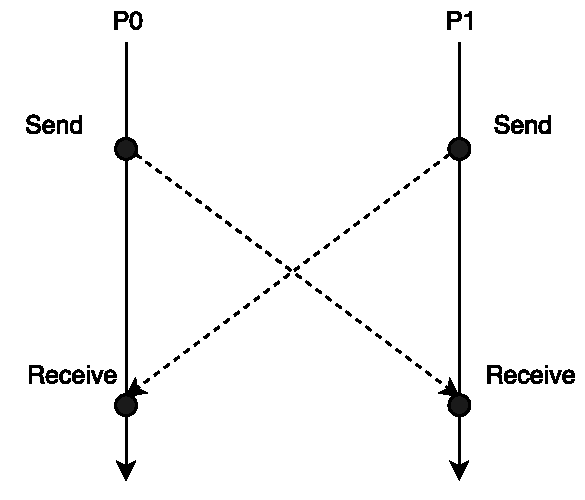
\includegraphics[width=7cm,height=6cm]{example.jpg}
		\centerline{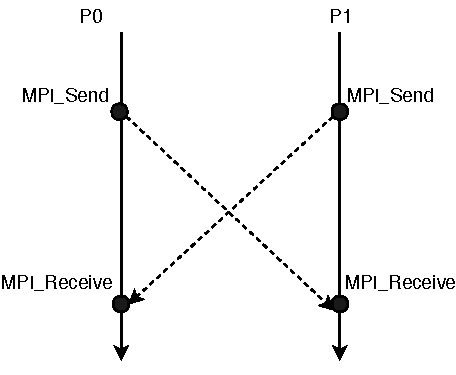
\includegraphics[width=7cm,height=6cm]{mpiPro.pdf}}

	\caption{A MPI program with a potential deadlock}
\end{figure}
In SimGrid, actions are atomic and actions in the same actor are totally ordered, but actions in the whole system are partially ordered (partial order relation).  Hence, there are different instances (runs) of the system, and the relation between actions are  considered in a given instance. A global state is defined as a set of local states of the actors, states of the $Mailboxes$, states of the $Mutexes$ and state of the \Communications. Function execute($S_i$,t)  gives the next global state after executing transition t in the state $S_i$ while function $getEnabled(S_i)$
gives all the enabled transitions at state $S_i$. We define function $pre(a)$ giving the immediate precede action of $a$ in the same process.\\

 To adapt to the reality, happened-before relation in SimGrid is flexible. Let's look at an example in Figure~\ref{fig:cycle_dependency}. A MPI program including two processes, and process P0 sends a massage to process P1 (doted line). Before receiving  the massage from P0, P1 also sends a massage to P0. At first glance, we may think that there is a deadlock in the program since there is a dependency cycle. However, in practice, depending on the size of the massages exchanged by the processes, the deadlock may appears or not. MPI\_Send and MPI\_Receive are blocking functions in MPI, but they may or may not block. MPI\_Send is ambiguously define, it will not return until the buffer passed to it can be reused. For sending small enough massages, those massages eagerly sent before the calling MPI\_Receive from receiving processes (eager protocol). Hence, MPI\_Sends are not blocked until matching MPI\_Receive have been posted. Actually, if the massages are small, MPI can easily find spaces in internal storage to save them before they are really sent. On the other hand, working with large massages, blocking communications are used, MPI\_Sends must wait for matching MPI\_Receives. Therefor, the scenario in Figure~\ref{fig:cycle_dependency} may or may not has a deadlock. SimGrid covers both cases, users can chose optionally two modes detecting or not deadlocks in the same situation with the above scenario. This conversion can be done easily by switching between two happened\_before definitions.    
  \begin{definition}
  	\label{def:happedBefore1}
  The happened-before relation  denoted by  $\rightarrow $ can be defined based on two relations precede and causality: \begin{itemize}
  	\item Immediate precede (denoted by $ \prec$) :  Two actions e and f in the same actor $A_i$, e $ \prec$ f if the occurrence of e precedes the occurrence of f in the actor $A_i$  
  	\item Remotely precede (denoted by $\leadsto$): Action e is the \asynsend~ or \asynreceive~ action of actor $A_i$, action f is the Wait action of the actor $A_j$,  e $\leadsto$ f if e and f concerns the same communication request.
  	\item The ‘happened before’ is a transitive relation including immediate precede and remotely precede. 
  \end{itemize}\end{definition} 
  
 \begin{figure}[H]
\label{fig:hapend_before}
\subfigure[deadlock]{
		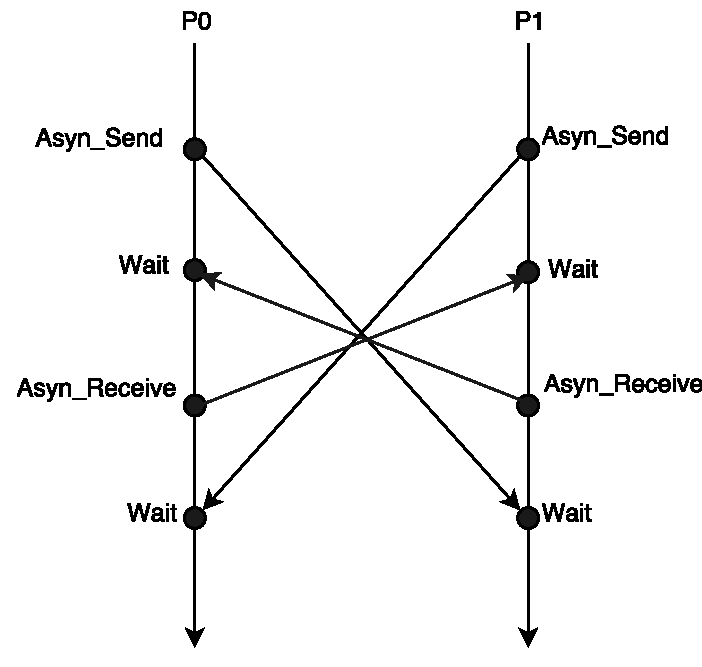
\includegraphics[width=7cm,height=7cm]{deadlock.pdf}
	}
\hfill
\subfigure[dealock free]{
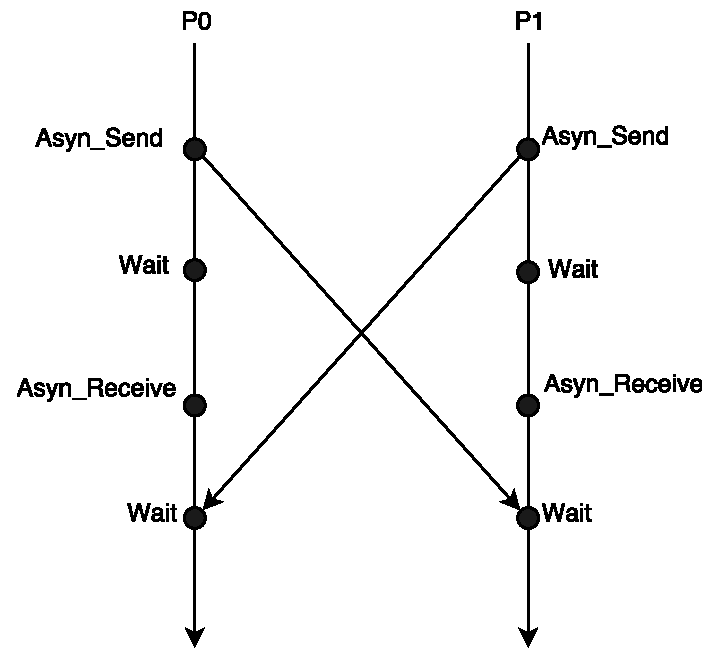
\includegraphics[width=7cm,height=7cm]{deadlockFree.pdf}
	}
\caption{Happened- before relations between actions}
\end{figure}

The diagram in Figure~\ref{fig:hapend_before}(a) illustrates happened\_before relations (denoted by arrow lines) between actions in the program based on Definition~\ref{def:happedBefore1}. In SimGrid a MPI\_Send is simulated by a \asynsend~ and a \wait~ while a MPI\_Receive comprises a \asynreceive~ and a \wait. Obviously, there is a happened\_before relation cycle in the diagram; the cycle includes the first \wait~ and \asynreceive~ of P0, the first \wait~ and the \asynreceive~ of P1. The existing of cycle leads to a deadlock in the program. In the case we do not want to capture the deadlock, Definiton~\ref{def:happedBefore2} is used.

\begin{definition}
  	\label{def:happedBefore2}
  The happened-before relation  denoted by  $\rightarrow $ can be defined based on two relations precede and causality: \begin{itemize}
  	\item Immediate precede (denoted by $ \prec$) :  Two actions e and f in the same actor $A_i$, e $ \prec$ f if the occurrence of e precedes the occurrence of f in the actor $A_i$  
  	\item Remotely precede (denoted by $\leadsto$): Action e is the \asynsend~action of actor $A_i$, action f is the Wait action of the actor $A_j$,  e $\leadsto$ f if e and f concerns the same communication request.
  \item The ‘happened before’ is a transitive relation including immediate precede and remotely precede.
  \end{itemize}\end{definition} 

Using Definition~\ref{def:happedBefore2} and presenting the happened\_before relation between actions of the program in Figure~\ref{fig:hapend_before}(b), we can see that there are no any cycle, then the program is deadlock-free.

The happened-before relation is not a total order on the actions, two actions may not related by a happened-before relation. In that case, we say that they are concurrent denoted by the symbol $\parallel$. For example, in the above figures, since $\neg$(\asynsend~ of P0 $\leadsto$ \asynsend~ of P1) and $\neg$(\asynsend~ of P0 $ \prec$  \asynsend~ of P1 ) then \asynsend~ of P0 $\parallel$ \asynsend~ of P1.  
\subsection{Event structures}
\textit{Labelled Prime Event Structure (PES for short).} This section recaps the definition of labelled event structures~\cite{DBLP:conf/concur/RodriguezSSK15}

\begin{definition} A labelled event structure on a set label L is a tuple  $\mathpzc{E}$ = $\langle E,<,\#,h \rangle$ where
 \begin{itemize}[noitemsep]
 	\setlength{\itemsep}{2pt}
\item E is a set of events.
\item $<$ is a partial order relation on E, called causality relation.
\item h : E $\rightarrow$ L is a labeling function assigning each event in E to a label in L. 
\item  $\#$ is an irreflexive symmetric relation called conflict relation such that for every event e $\in$ E, the set causes(e) = \{ e' $\in$ E: e'$<e$\} is finite (the set of predecessors of e is finite), and for every events e, f, g $\in$ E, if e \# f and g $<$ f then e \# g.
\end{itemize}
\end{definition}
 Intuitively, the causality relation expresses the happened-before while two events are $conflict$ if they are not in one executions. Each label in L is an action, and if two events neither are $conflict$ nor $causality$ related, they are $concurrent$. An important notion in PESs is $configuration$. A subset of events C of E is a \textit{configuration} if for every event e $\in$ C, $causes(e)$ $\subseteq$ C (all events in causes of e belong to C) and $\forall e, e' \in C, \neg(e \# e')$ (there is no conflict relation in C). We use $Conf(\mathpzc{E})$ to present the set of all configuration in $\mathpzc{E}$.
 
 \section{Unfolding Structure}
 \MQ{Rephrase it to fit our new way of presenting things}
 \textit{Unfolding Semantics (Unfolding for short).} Unfolding Semantics is proposed in~\cite{DBLP:journals/corr/abs-1802-03950} and can describe behavior of a distributed system under dependence relations. Indeed, a unfolding is a LES where each maximal configuration corresponds to a Mazurkiewicz trace. In the $unfolding$, each event e is presented by a pair e = $\langle a, H \rangle$ where $a$ is an action in $M_P$, and H is a history of e denoting that event e occurs after all events in H. For a given configuration C, an event e is called maximal event of C if $\nexists$ e' $\in$ C such that e $<$ e'. Let MaxEvt(C) is a set comprised of all maximal events of C. Formally, MaxEvt(C) = \{e $\in$C : $\nexists$ e' $\in$ C and e $<$ e' \}; For event e = $\langle a, H \rangle$ and event e' = $\langle a', H' \rangle$, function immediate precede $pre(e) = e'$ if only if $pre(a) = a'$. For a given distributed system P and independence relations in $M_P$, the method in~\cite{DBLP:journals/corr/abs-1802-03950} can be applied to build the unfolding of the distributed system P (denoted by $U_P$) as follows:
\begin{enumerate}
\item The unfolding $U_P$ = $\langle E,<,\#,h \rangle$  starts with $\langle \emptyset, \emptyset, \emptyset,\emptyset \rangle$.
\item Repeating two following steps until we can not add any new events to E.
\item For each configuration C $\in$ conf($U_P$), and for each action a $\in$ L, add a new event e =  $\langle a , C \rangle$ to E if D(a, h(e')) holds for all e' $\in$ MaxEvt(C) and 
\begin{itemize}
 \item if the action $a$ $\in$ \{ \asynsend, \asynreceive, \test, \mutexlock, \mutexunlock, \mutextest \} then $pre(e)$ $\in$ C
 \item if action $a$ is a \mutexwait($A_i, m_j$) action then $pre(e)$ $\in$ C and the actor $A_i$ must be the owner of the mutex $m_j$. 
 \item if action $a$ is a \wait~then  then $pre(e)$ $\in$ C and the communication tested by the \wait~must has a "ready" status. 
\end{itemize}
\item Updating $<$, $\#$ and h as following: e' $<$ e if  e $\in$ C; e' \#  e if D(a, h(e') and e' $\in$ E $\setminus$C; h(e) = $a$.\\   
\end{enumerate}
Figure~\ref{fig:unfoldSematics} displays a distributed program P composed of three actors. Actor0 and Actor2 send \asynsend~requests to the mailBox1 while Actor1 posts a \asynreceive~to the mailBox1. After sending the request, Actor0 wait the request by firing a \wait~command. The unfolding of the program is described in the right of Figure~\ref{fig:unfoldSematics}. At initial step (denoted by \#) $U_P$ = $\langle \emptyset, \emptyset, \emptyset,\emptyset \rangle$. There is only one configuration C = $\emptyset$ in $Conf(U_p)$. After that events 1 = $\langle \asynsend, \emptyset \rangle$, 2 = $\langle \asynreceive, \emptyset \rangle$ and 3 = $\langle \asynsend, \emptyset \rangle$ are created. We create those events because they have not  precede events, and there is no maximal event in  C to check the dependence condition. We now have four configurations \{1\}, \{2\}, \{3\}, \{1, 2\}, \{2, 3\} and $\emptyset$. For the configuration \{1, 2\} we can create event 6 since $pre(6)$ = 1 (1 $\in$ \{1, 2\}), the communication is now ready, and \wait~is dependent with h(1) and h(2). Similarly, we have event 4, 5, 7 and 8. Note that, we have a configuration \{2, 3, 8\}, and h(2) h(8) (they are maximal events) are dependently related to \wait; however, we can not create a new event by combining that configuration with action \wait~because the communication $com$ is not ready for processing.

\begin{figure}[H]
\label{fig:unfoldSematics}

\begin{multicols}{2}



\centering
\begin{tabular}{c c}
	\\\\
\code{Actor0:}&\code{com = AsynSend(mailBox1) }\\&\code{Wait(com)} \\\\
\code{Actor1:}&\code{AsynReceive(mailBox1)} \\\\\\
\code{Actor2:}&\code{AsynSend(mailBox1)} \\
\end{tabular}
\label{table:ta}
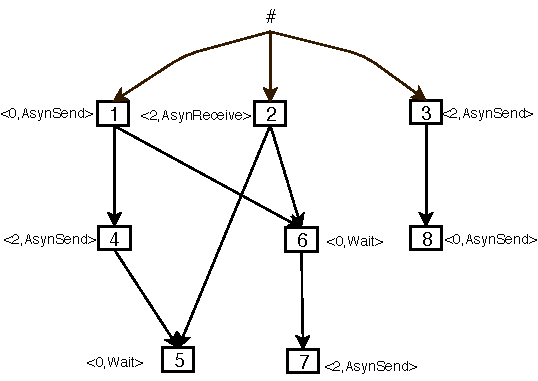
\includegraphics[width=\linewidth]{unfolding.pdf}

\end{multicols}
\caption{A (toy) program (left), and it's unfolding  semantics (right)}

\end{figure}


\section{MPI Implementation}\label{sec:mpi}
TODO: explain here how MPI is implemented on top of the previously described API
\newpage
\nocite{*}	  	
\bibliographystyle{alpha}
\bibliography{Reference}

%%%%%%%%%%%%%%%%%%%%%%%%%%%%%%5
\begin{appendices}
\begin{theorem} Two \mutexlock~actions are independent if they concern different mutexes.\\  $\forall  p_1, p_2 \in Proc $; $m_1, m_2 \in $ Mutex : $p_1 \ne p2, m_1 \ne m_2 	\Rightarrow $ I(lock($p_1,m_1$), lock($p2, m_2$) )
\end{theorem}

 \textbf{Proof}: We will prove that the theorem satisfy both conditions of the Definition 1. We start with the first condition. Suppose both lock($p_1,m_1$) and lock($p_2, m_2$) operations are enabled at the state \\
  s = $\langle network, memory, pc, pcState, waitedQueue	\rangle$. We will prove that executing these operations in either orders lead to the same state. Indeed, depending on the value of waitedQueue[m1], firering lock($p_1,m_1$) lead to two cases: 
  \begin{itemize}
  	\item  if waitedQueue[$m_1$] is empty, we have  $s\xrightarrow{\text{lock($p_1, m_1$)}}s_1$ where $s_1$ = $\langle$ network, memory, $pc_1$, pcState,$waitedQueue_1$ $\rangle$ in which the queue waitedQueue[$m_1$] = \{$p_1$\}. At the state $s_1$, the mutex $m_1$ is occupied by the process $p_1$, while network and memory and pcState remain their value, and the only one possible change in the array pc (program counter) is pc[$p_1$].
  
  	\item if waitedQueue[$m_1$] is not empty then $s\xrightarrow{\text{lock($p_1, m_1$)}}s'_1$ where $s'_1$ = $\langle$ network, memory, $pc_1$, $pcState'_1$, $waitedQueue'_1$ $\rangle$ where $pcState'_1[p_1]$ = "blocked" since there is another process already occupied the mutex $m_1$, and  $waitedQueue'_1[m_1]$ = Append(waitedQueue[m1]), $p_1$) ($p_1$ will be added to waitedQueue[m1] to form the queue $waitedQueue'_1[m_1]$). Like the case above pc can be changed to $pc_1$, the other variables network and memory remain stable since the operation lock does not intervene their values.  
  \end{itemize}
  
  In the both cases, only one difference between pc and $pc_1$ is that the value of program counter of process $p_1$ can be changed to another instruction. At the both state $s_1$ and $s'_1$, the lock($p_2, m_2$) is still enabled, since the value of pc[$p_2$] and pcState[$p_2$] do not change. Now fire the lock($p_2, m_2$) from the two state $s_1$ and $s'_1$:
  \begin{itemize}
  	\item Like the situation when we execute lock($p_1, m_1$), firering the operation lock($p_2, m_2$) on $s_1$ can lead to two cases:
	  	\begin{itemize}
			\item  if $waitedQueue_1[m_2]$ is empty, we have $s_1\xrightarrow{\text{lock($p_2, m_2$)}}s_2$ where  $s_2$ = $\langle$ network, memory, $pc_2, pcState, waitedQueue_2 \rangle$ and waitedQueue[$m_1$] = \{$p_2$\}
			\item if $waitedQueue_1[m_2$] is not empty, we have $s_1\xrightarrow{\text{lock($p_2, m_2$)}}s'_2$ where  $s'_2$ = $\langle$ network, memory, $pc_2, pcState'_2, waitedQueue' \rangle$ and $pcState'_2[p_2]$ = "blocked" since there is another process already occupied the mutex $m_1$, and  $waitedQueue'_1[m1]$ = Append(waitedQueue[m1]), $p_1$) ($p_1$ will be added to waitedQueue[$m_1$] to produce a new queue $waitedQueue'_1[m1]$). 
	  	\end{itemize}
	\item Similarly, depending on the value  of $waitedQueue'_1[m_2]$, executing lock($p_1, m_1$) from $s'_1$ results in two possible states $s_3$ and $s'_3$ :
	
  	  \begin{itemize}
  	  	\item  $s'_1\xrightarrow{\text{lock($p_2, m_2$)}}s_3$ where $s_3$ = $\langle network, memory, pc_3, pcState'_1, waitedQueue_3 \rangle$ and $p_2$ will be the owner of the mutex $m_2$ ( $waitedQueue_3$[$p_2$] = \{ $p_2$\}) while state of all processes do not change compared to their values in the previous state (the state $s'_1$)
  	  	  	  	  	
  	  	\item  $s'_1\xrightarrow{\text{lock($p_2, m_2$)}}s'_3$ where $s'_3$ = $\langle network, memory, pc_3, pcState'_3, waitedQueue'_3 \rangle$, and $p_2$ will be queued to the queue of $m_2$ ($waitedQueue'_3$[$p_2$] = Append($waitedQueue'_1 ,p_2$) while the process $p_2$ will be blocked ($pcState'_3[p_2]$ = "blocked"). 
  	  \end{itemize}
  \end{itemize}
 From above executions, starting from the state s, by firering lock($p_1,m_1$) before  lock($p_2, m_2$), we have four possible outcome states and scenarios:  $s\xrightarrow{\text{lock($p_1, m_1$)}}s_1 \xrightarrow{\text{lock($p_2, m_2$)}}s_2$, $s\xrightarrow{\text{lock($p_1, m_1$)}}s_1 \xrightarrow{\text{lock($p_2, m_2$)}}s'_2$, $s\xrightarrow{\text{lock($p_1, m_1$)}}s'_1 \xrightarrow{\text{lock($p_2, m_2$)}}s_3$, $s\xrightarrow{\text{lock($p_1, m_1$)}}s'_1 \xrightarrow{\text{lock($p_2, m_2$)}}s'_3$. In the opposite order, executing lock($p_1,m_1$) after lock($p_2, m_2$) we also get four possible outcome states and scenarios, and they are equal in pairs. Hence, the property is satisfied. \\
 
 Concerning second condition, based on the proof of the first condition, we can realize that firering one operation does not change values which need for enable the other operation. Indeed, if at the state s = $\langle network, memory, pc, pcState, waitedQueue \rangle$ we fire lock($p_1,m_1$) the values of pc[$p_2$] and pcState[$p_2$] do not change. Hence, if lock($p_2,m_2$) is enabled at state s' ( $s\xrightarrow{\text{lock($p_1, m_1$)}}s'$) if only if it is enabled in s. 
\end{appendices}

\end{document}